\documentclass[11pt]{article}
\usepackage{hyperref}

\usepackage{amsmath, verbatim}
\usepackage{amssymb}
\usepackage{fancyhdr}
\usepackage{pstricks}
\usepackage{pstricks-add}


\setlength{\oddsidemargin}{0.0in}
\setlength{\evensidemargin}{0.0in}
\setlength{\textheight}{8.4in}
\setlength{\textwidth}{6.5in}
\setlength{\voffset}{0.00in}
\setlength{\headsep}{26pt}
\setlength{\parindent}{0pt}
\setlength{\parskip}{6pt}

% header information
\pagestyle{fancyplain}
\lhead{MATH 150: Wednesday January 27}
\rhead{\textit{Spring Semester 2021}}


\usepackage{graphicx} %m\'ethode pour ins\'erer des images version net
\DeclareGraphicsExtensions{.eps,.pdf,.png,.jpg,.JPG,.jpeg,.ps,.svg}
%\usepackage{graphicx}
\chead{\textbf{Homework 8: individual}}

\begin{document}

{\bf Submit your work on Catcourses by April 21st at 11:59pm}

%\begin{itemize}
%\item Be familiar with notebook
%\item scales, create simple models maybe
%\item dynamical systems a little bit ? 
%\end{itemize}
\begin{enumerate}
%\item We want to model the growth of mosquito bites over the summer in Merced. Let's denote $y_k(t)$ the total number of bites after $t$ days of the $kth$ person. Let's consider the simplest model, the linear growth model:
%\[ y_k'(t) = \lambda y_k(t), \quad y_k(0) = \alpha, \quad k = 1, \dots, N,  0 \leq t \leq 30.\]
%\begin{enumerate}
%\item What is the expression of the solution of this ODE  ?
%\item Data after $t = 30$ days has been collected and stored as $(k,y_k)$, $k = 1, \dots, 100$, given in the {\tt hwk5\_data.csv} file. But there is some noise in the data. We assume that the growth rate $\lambda $ follows a normal distribution $\mathcal{N}(\mu, \sigma)$. This means that the probability to observe $\lambda = \lambda_i$ is given by $p(\lambda_i, \mu,\sigma) = \frac{e^{-(\lambda_i -\mu)^2/{2 \sigma}}}{\sqrt{2 \pi \sigma}} $, and the maximum likelihood for $\mu$, $\sigma$ is given by (as done in class) is $ \mathcal{F}(\mbox{data}) = \prod \limits_{i=1}^{100} \frac{e^{-(\lambda_i -\mu)^2/{2 \sigma}}}{\sqrt{2 \pi \sigma}} $. If $\lambda$ is a random variable following a normal distribution, using the expression of $y$, find the expression of the observations $\lambda_i$.
%\item For $\alpha = 2$, using the data, and the lecture notes, find the MLE for $\mu$ and $\sigma$. How accurate are your estimates ?
%\end{enumerate}
\item The Susceptible-Infectious-Recovered (SIR) model is a well-known compartmental model that can be used to model disease spread, epidemics, etc. It can also be modeled as a Markov chain:
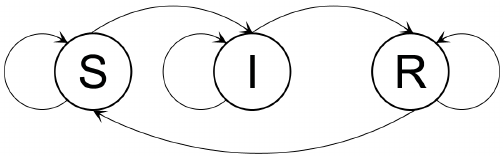
\includegraphics[width=0.5\linewidth]{SIR.png}
\begin{enumerate}
\item Associate values (your choice BUT justify it) to each transition from the graph above and write the associate Transition matrix $\mathcal{P}$. 
\item Suppose we use the SIR model to simulate the \textit{Math 150 fever}: this infectious disease makes any infected person model everything all the time (write equations everywhere even on their body, simulate everything even on their smart phone, question every single aspect of their lives and discussing it with any encountered person). The above Markov chains the represents the transition to all states in a day time. Suppose that the current Math 150 class is distributed as follows: 60\% susceptible, 10\% infected, and 30\% recovered. With your chosen values, what would happen after a semester (75 class days) ? You can change the values chosen in the previous question, as long as you explain your reasoning.
\end{enumerate}
{\item Submit your work on Catcourses under the assignment \texttt{Homework 8 (individual)} \textbf{as a .ipynb}}. 
\end{enumerate}


%In the file {\tt HW1\_xvec.mat} you will find data relevant for this homework.
%
%You may load this data, and plot it, into Matlab using the following commands:
%\begin{verbatim}
%data = load('HW1_xvec.mat');
%plot(data.x,data.y1)
%plot(data.x,data.y2)
%xshort = data.x(1:100);
%y3short = data.y3(1:100);
%plot(xshort,y3short)
% \end{verbatim}  
%  
% \begin{enumerate}
% \item Define two simple weather models that predict daily temperature and rainfall. Compare those models with commercial predictions and actual weather every day for one week, and assess which models performed best. Justify your rankings.
% 
% \item Try to determine the best possible function to fit the data $y_1$, which represents a function of the data in $x$ (that is for every index $i$, $y_1^i = f_1(x^i)$). Indicate what functions you tried (even the ones that were not the best) and how you determined which function was the best. Be sure to consider both small and large values of $x$.
% \item  Try to determine the best possible function to fit the data $y_2$, which represents a function of the data in $x$. Indicate what functions you tried (even the ones that were not the best) and how you determine which function is the best. Be sure to consider both small and large values of $x$.
% \item  Try to determine the best possible function to fit the data $y_{3short}$, for the first 100 entries of $y_3$ which represents a {\bf periodic} function of the first 100 entries in $x$. Indicate what functions you tried (even the ones that were not the best) and how you determine which function is the best.
% \end{enumerate}
   
% y1 = 3*x.^2 + 4./x + 0.01*sin(4*x) + 3;
% y2 = 2*log(x) - x/3;
% y3 = cos(7*x*2*pi) + 3*sin(x*2*pi) + 0.5*sin(4*x*2*pi);
% for the first 100 entries only, periodic afterwards


\end{document}
